\documentclass[11pt, letterpaper]{article}
\usepackage[utf8]{inputenc} %Paquete de Codificación
\usepackage[spanish]{babel} %Paquete de idioma
\usepackage{enumitem}       %Paquete para listas
\usepackage{graphicx}       %Paquete para imagenas
\usepackage{amsmath}        %Paquete para matematicas
\usepackage{lipsum}         %Paquete para texto aleatorio
\usepackage{hyperref}
\usepackage{listings}
\graphicspath{ {img/} }  %Path para carpeta imagenes









\begin{document}
    
\begin{titlepage}
    \centering
    {\bfseries\LARGE Universidad de Alicante\par}
    \vspace{1cm}
    {\scshape\Large Escuela Politecnica Superior\par}
    \vspace{3cm}
    {\scshape\Huge Entregable 2\par}
    \vspace{3cm}
    \vfill
    {\Large Autor: \par}
    {\Large David Carbonell Pastor \par}
    \vfill
    {\Large 2022\par}
    \end{titlepage} 

\tableofcontents

\pagebreak

\section{Uso de la plataforma IoT Ubidots}
\subsection{Evidencias del trabajo realizado}
Se ha utilizado la plataforma IoT Ubidots a través de Node-Red como se puede ver en la figura \ref{fig:ubidots_nodered}
de esta manera se simplifica el apartado de la programación ya que de otra manera se ha de realizar mediante codigo python para 
lo que pretendemos implementar.
\begin{figure}[h]
    \centering
    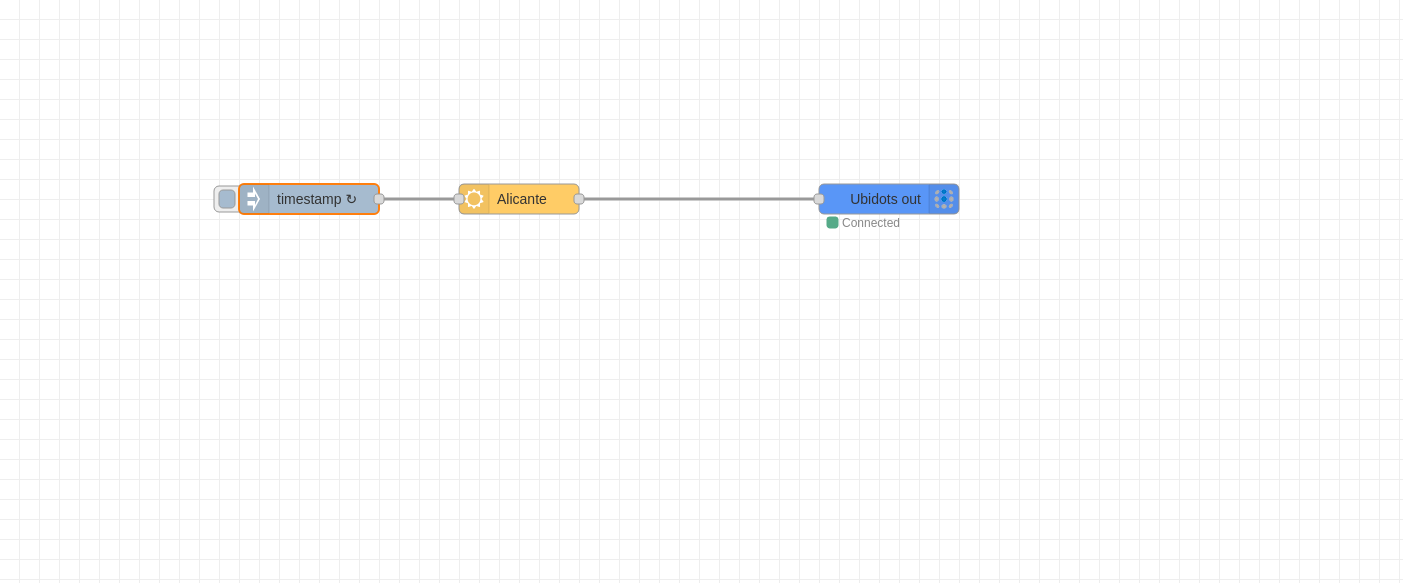
\includegraphics[width=\textwidth]{ubidots_nodered.png}
    \caption{Conexion de ubidots con nodered}
    \label{fig:ubidots_nodered}
\end{figure}

Enviamos la información del nodo de openweather al nodo de ubidots 
en la pagina de ubidots en el apartado devices nos aparecen los parametros 
que nos proporciona en formato json de una manera mas visual donde podemos ver los 
distintos datos que tenemos.\\


Con los datos proporcionados por el nodo de openweather se ha realizado un dashboard simple \ref{fig:dashboard_ejemplo}
el cual presenta una menor complejidad y mayores funcionalidades que los dashboard creados con node-red 
en el anterior entregable.
\pagebreak
\begin{figure}[h]
    \centering
    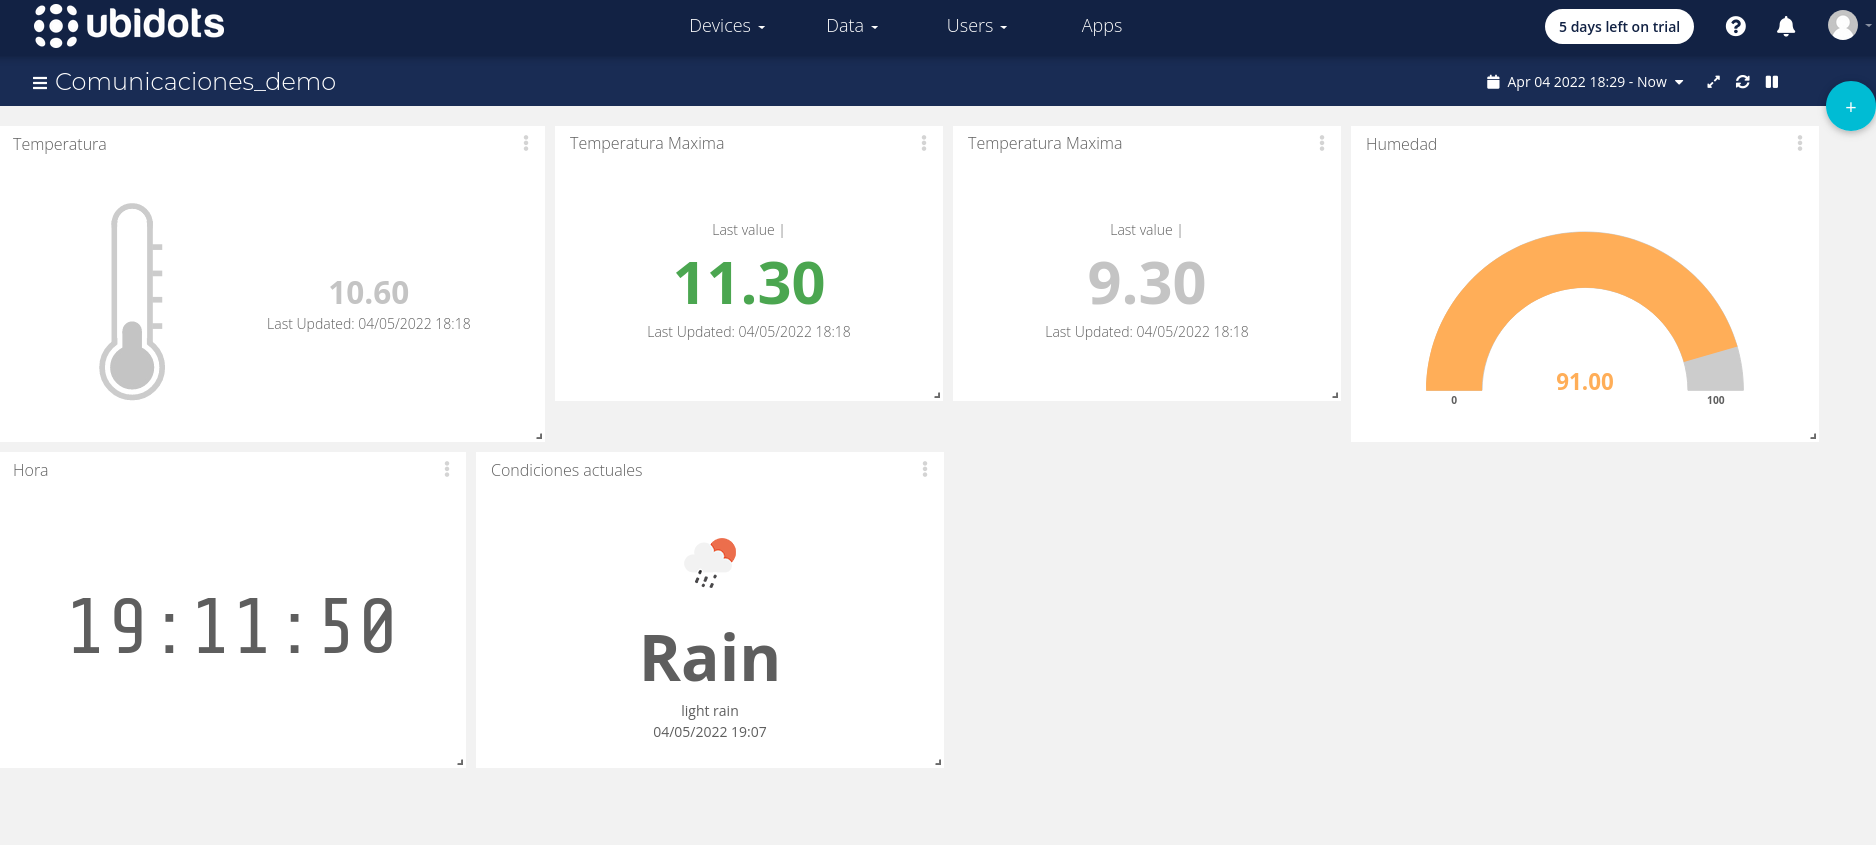
\includegraphics[width=\textwidth]{dashboard_ejemplo.png}
    \caption{Dashboard simple con datos de openweather}
    \label{fig:dashboard_ejemplo}
\end{figure}


\end{document}